\section{Trees and tree-to-tree functions}
\label{sec:trees-transductions}
 In this section, we describe the trees and tree-to-tree functions that are discussed in this paper. The  trees are rooted, node labelled, ranked (the label of a node determines the number of children) and sibling ordered (there is a first child, second child, etc.). 
A \emph{ranked set} is a set where each element has an associated \emph{arity} in $\set{0,1,2,\ldots}$. We adopt the convention that ranked sets are written in red, e.g.~$\rSigma$ or $\rGamma$.  We use ranked sets as building blocks for trees. The following picture describes the notion of trees that we use and some terminology:\\
\begin{center}
\includegraphics[scale=.35]{ranked-tree.pdf}
\end{center}

% When talking about elements of a ranked set, we mean elements of the underlying set.   For a ranked set $A$ and a finite set of variables $X \subseteq \varnames$, we write $\slice A X$ for the elements of $A$ that have arity $X$. 

We use standard tree terminology, such as ancestor, descendant, child, parent. We write $\trees \rSigma$ for the set of trees over a ranked set $\rSigma$. This paper is about \emph{tree-to-tree functions}, which are functions of the type \begin{align*}
f : \trees \rSigma \to \trees \rGamma.
\end{align*}
%We also discuss tree languages, i.e.~sets of trees. 
%A tree language can be viewed as the special case of a tree-to-tree function, where the output alphabet $\Gamma$ contains only two letters ``yes'' and ``no'' of arity zero. Later on, we will also discuss terms, which are trees with variables. 

  
\subsection{First-order logic and transductions}
In this section we  describe how logics -- such as first-order logic or monadic second-order logic -- can be used to define tree-to-tree functions and tree languages. The basic idea is to view a tree as a model, and to use logic to describe properties and transformations of such models\footnote{For more about these logics in the context of defining properties of trees, see~\cite[Section 3]{thomas1997languages}.}. 

A \emph{relational vocabulary} is defined to be a set of relation names, each one with associated arity (we do not use function symbols in this paper). Formally speaking, a relational vocabulary is the same as a ranked set, which is why we write relational vocabularies in red, using letters like $\ranked \sigma, \ranked \tau$. 

\begin{definition}[Tree as a model]\label{def:tree-model}
   For a tree $t$  over a ranked alphabet $\rSigma$, its \emph{associated model} $\underline t$ is defined as follows. The  universe is the nodes of the tree, and it is equipped with the following predicates:
   $$\begin{array}{lcl}
   x<y & : &   \text{$x$ is an ancestor of $y$} \\
   \mathrm{child}_i(x) & : & \text{$x$ is an $i$-th child (for each $i\in \set{1,2,\ldots}$)} \\
   a(x) & : &   \text{$x$ has label $a$ (for each $a \in \Sigma$)}
   \end{array}$$
    \end{definition}

The $i$-th child predicates are only needed for $i$ up to the maximal arity letters in the ranked alphabet, and hence the vocabulary in the above definition is finite. 
 A sentence of first-order logic (or of \mso)  over this vocabulary   describes a tree language, namely the set of trees whose associated models satisfy the sentence.  For example, the sentence 
 \begin{align*}
 \forall x \ a(x) \Rightarrow \exists y \ x < y \land b(x)
 \end{align*} 
 is true in (the models associated to)  trees $t$ where every node with label $a$ has a descendant with label $b$.  
 
 \paragraph*{Tree-to-tree functions.}
 Apart from defining yes/no properties, first-order logic can also be used  to define transformations on  models. In the context of this paper, we are interested in first-order transductions%\footnote{   First-order transductions are  a special case of a first-order interpretations~\cite[p.~213]{hodges_model_1993}, which use tuples (instead of elements) in the input structure to describe elements in the output structure. As a result, first-order transductions have linear size increase, while first-order interpretations have polynomial size increase. First-order transductions are also a special case of \mso transductions, see~\cite[Section 7]{courcelle_graph_2012}, which use \mso logic instead of first-order logic, and which also allow a step where the input structure is nondeterministically coloured (and therefore the result is a binary relation on structures which is not necessarily functional).}
, defined below. 

\begin{definition}[First-order transduction]\label{def:fo-transduction}~\\[-10pt]
%\begin{enumerate}
 %   \item 
 

 1. \emph{Copying.} Fix some  relational vocabulary $\ranked \sigma$ and let $k \in \set{1,2,\ldots}$. Define $k$-copying to be the operation 
    $$\begin{array}{lll}
     \text{models over $\ranked \sigma$} & \to & 
     \begin{array}{c}
     \text{models over $\ranked \sigma$}\\ 
     \text{extended with a $k$-ary relation $\mathrm{copy}$}
     \end{array}
    \end{array}$$
which inputs a model $\mathbb A$, and outputs $k$ disjoint copies of $\mathbb A$, where the  $\mathrm{copy}$ relation is interpreted as the set of tuples $(a_1,\ldots,a_k)$ such that, for  some $a \in \mathbb A$, the first copy of $a$ is  $a_1$, the second copy of $a$ is $a_2$, etc. The $\mathrm{copy}$ relation  is not commutative, because we distinguish the copies.
\smallskip

2.    \emph{Non-copying first-order transduction.} The syntax of a \emph{non-copying first-order transduction}  is given by:
\begin{enumerate}
    \item Input relational vocabulary $\ranked\sigma$ and output relational vocalbulary $\ranked{\gamma}$.
    \item A first-order \emph{universe formula} $\varphi(x)$ over $\ranked{\sigma}$.
    \item For every relation $R$ in vacubulary $\ranked{\gamma}$, a first-order  formula $\varphi_R(x_1,\ldots,x_{\arity R})$ over $\ranked{\sigma}$.
\end{enumerate}
The semantics of a non-copying first-order transduction is  a function
\begin{align*}
    \text{models over $\ranked\sigma$} \quad \to \quad \text{models over $\ranked\gamma$}
\end{align*}
defined as follows. If the input model is $\mathbb A$, then the output model is defined as follows: the universe is elements of $\mathbb A$ which satisfy the universe formula, and each relation $R$ is interpreted as those tuples that satisfy $\varphi_R$. 

\smallskip
3. \emph{First-order transductions.} A \emph{first-order transduction} is defined to be any  composition of $k$-copying (for some $k$) followed by a non-copying first-order transduction. 
% \end{enumerate}
\end{definition}



Every first-order  transduction has linear size increase, i.e.~if the input structure has a finite universe of size $n$, then the output structure has a universe of size at most $kn$, where $k$ is the number of copies used in the transduction. First-order transductions are easily seen to be closed under composition.

\begin{definition}[First-order tree-to-tree transduction.]
    A \emph{first-order tree-to-tree transduction} is any tree-to-tree  function which can be implemented by a first-order transduction, assuming that trees are modelled according to Definition~\ref{def:tree-model}. More formally, a first-order tree-to-tree transduction is any function $f$ which makes the following diagram commute
    \begin{align*}
        \xymatrix{
            \trees \rSigma \ar[d]_{t \mapsto \underline t}\ar[r]^f & \trees \rGamma \ar[d]^{t \mapsto \underline t} \\
            \set{\underline t : t \in \trees \rSigma} \ar[r]_g & \set{\underline t : t \in \trees \rGamma}.
        } 
    \end{align*}
for some first-order transduction $g$.     
\end{definition}


There are also \mso tree-to-tree transductions, these will be discussed later, in Section~\ref{sec:mso-trans}.  We conclude this section with an example of first-order tree-to-tree transduction. A more elaborated example could be found in Appendix~\ref{sec:appendix-example-fo-transductions}.

\begin{example}
    Let the input and output alphabets be:\vspace{-15pt}
    \mypic{17}
    and consider the tree-to-tree function which removes the unary nodes:
\begin{center}
\includegraphics[scale=.35, page=19]{pics.pdf}
\end{center}
This is a first-order tree-to-tree transduction, which needs no copying (formally speaking, it uses 1-copying). The domain formula selects nodes which have non-unary labels, and the descendant relation is inherited from the input tree. To define the child relation on the output tree, we need to use the descendant relation in the input tree. A node $x$ in the input tree is an $i$-th child in the output tree if it satisfies the following first-order formula:
\begin{align*}
    \exists y \ \child i (y) \land \underbrace{y \le x \land   \forall z\ (y < z < x \Rightarrow \blueball(z))}_{\substack{\text{$y$ is the farthest ancestor that can be} \\ \text{reached from $x$ using only unary nodes}}}
\end{align*}
%This function could not be implemented by a first-order transduction if we replaced the descendant relation by a binary parent-child relation.
\end{example}

